\documentclass[journal,10pt,twocolumn]{article}
\usepackage{graphicx}
\usepackage[margin=0.5in]{geometry}
\usepackage[cmex10]{amsmath}
\usepackage{array}
\usepackage{booktabs}
\usepackage{listings}
\title{\textbf{Optimization Assignment - Advanced}}
\author{Bhavani Kanike}
\date{October 2022}

\providecommand{\norm}[1]{\left\lVert#1\right\rVert}
\providecommand{\abs}[1]{\left\vert#1\right\vert}
\let\vec\mathbf
\newcommand{\myvec}[1]{\ensuremath{\begin{pmatrix}#1\end{pmatrix}}}
\newcommand{\mydet}[1]{\ensuremath{\begin{vmatrix}#1\end{vmatrix}}}
\providecommand{\brak}[1]{\ensuremath{\left(#1\right)}}

\begin{document}


\maketitle


\section*{Problem} Find the shortest distance between the following lines.\\
$\frac{x-3}{1} = \frac{y-5}{-2} = \frac{z-7}{1}$ and $\frac{x+1}{7} = \frac{y+1}{-6} = \frac{z+1}{1}$

\section*{Solution}
 From given question  \\
 We can write in terms of vector form of line:\\
\begin{center}
 	$L_1 : \vec{x} = \myvec{3\\5\\7} + \lambda_1\myvec{1\\-2\\1}$
\end{center}
\begin{center}
	$L_2 : \vec{x} = \myvec{-1\\-1\\-1} + \lambda_2\myvec{7\\-6\\1}$
\end{center}

We have \\
\begin{center}
	$L_1 : \vec{x} = \vec{a_1} + \lambda_1\vec{m_1} $
\end{center}
\begin{center}
	$L_2 : \vec{x} = \vec{a_2} + \lambda_2\vec{m_2} $
\end{center}
where, $\vec{a_i}, \vec{m_i}$ are positional and slope vectors of line $L_i$ respectively\\
Now, let us assume that $L_1$  and  $L_2$ are intersecting at a point. 
\\Therefore,\\
\begin{equation}
	\myvec{3\\5\\7} + \lambda_1\myvec{1\\-2\\1} = \myvec{-1\\-1\\-1} + \lambda_2\myvec{7\\-6\\1}
\end{equation}
\begin{equation}
	\lambda_1 \myvec{1\\-1\\1} - \lambda_2\myvec{7,-6,1} = \myvec{-1\\-1\\-1} - \myvec{3\\5\\7}
\end{equation}
\begin{equation}
	\myvec{1&7\\-2&-6\\1&1} \myvec{\lambda_1\\ \lambda_2} = \myvec{-4\\-6\\-8}
\end{equation}
Row reducing the Augmented matrix\\
\begin{equation}
	\myvec{1&7&-4\\-2&-6&-6\\1&1&-8} \rightarrow R_3 - R_1 \rightarrow\myvec{1&7&-4\\-2&-6&-6\\0&-6&-4}
\end{equation}
\begin{equation}
	\rightarrow R_2 + 2R_1 \rightarrow \myvec{1&7&-4 \\ 0&8&-14\\ 0&-6&-4}
\end{equation}
\begin{equation}
	\rightarrow R_3+\frac{3R_2}{4} \rightarrow \myvec{1&7&-4\\0&8&-14\\ 0&0&-\frac{29}{2}}
\end{equation}
Therefore the above matrix has $rank = 3$ ,Hence the lines do not intersect.Hence the lines $L_1$ and $L_2$ are skew lines\\\\
Let $d$ be the shortest distance between $L_1$ and $L_2$ and $\vec{p_1}$ and $\vec{p_2}$ be the positional vectors of its end points. \\
For $d$ to be the shortest , we know that\\
\begin{equation}
	\vec{p_1} = \vec{a_1} + \lambda_1 \vec{m_1}
\end{equation}
\begin{equation}
	\vec{p_2} = \vec{a_2} + \lambda_2 \vec{m_2}
\end{equation}

\begin{equation}
	d^2 = \norm{\vec{p_1} - \vec{p_2}} = (\vec{p_1} - \vec{p_2})(\vec{p_1} - \vec{p_2})^T
\end{equation}
\begin{equation}
	d^2 = (\vec{a_1 + \lambda_1 \vec{m_1} - \vec{a_2} - \lambda_2 \vec{m_2}})^2
\end{equation}

By substituting the values of $\vec{a_1}$ , $\vec{a_2}$ ,$\vec{m_1}$ and $\vec{m_2}$ in above equation we get a Quadratic equation in two variables $\lambda_1$ and $\lambda_2$\\
Therefore, the equation is given as follows

\begin{equation}
	d^2 = (4 + \lambda_2 - 7\lambda_2)^2 + (6 - 2\lambda_1 + 6\lambda_2)^2 + (8 + \lambda_1 -\lambda_2)^2
\end{equation}
\begin{equation}
	d^2 = 6\lambda_1^2 + 86\lambda_2^2 - 40\lambda_1 \lambda_2 + 116
\end{equation}
After solving the above equation we get the shortest distance between two lines\\


Therefore,
\begin{equation}
	Shortest Distance d = 10.77
\end{equation}\\\\


\section*{Execution}
Verify the above Solution in the following code.\\
\begin{lstlisting}
https://github.com/bhavani360/FWC_assignments
\end{lstlisting}
\bibliographystyle{ieeetr}
 

\section*{Construction}

\begin{figure}[h]
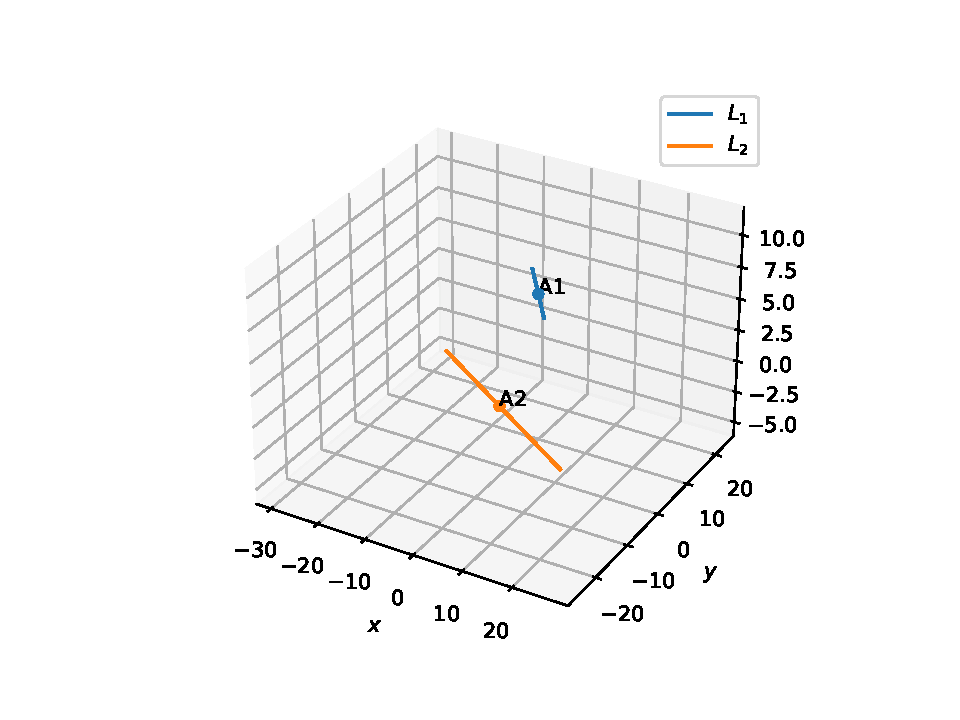
\includegraphics[scale=0.5]{opt_2.pdf} 
\end{figure}
\end{document}